% Recuperación aditiva: comunicados Witt v4--v7, tablas originales y
% RECUPERACION_ESTRELLAS_NONADICA_20260926. La procedencia completa está
% en el mapa editorial; el texto público conserva objetos y pruebas.
\subsection{Trois étoiles régionales et polarisation de leurs complétions}
\label{star27:comparacion}

La construction d'incidence précédente permet de comparer les régions au moyen d'une même opération. Les mots régionaux proviennent de l'émission APP--TRIT--TPK ; leur codage par \(\gamma_{A_W}(w)=(w,wA_W)\) conserve un support dans les douze positions. Le registre \(K\) et la cochaîne antérieure à la retenue ajoutent deux lectures du même état : la position par rapport à la frontière \(729+271\) et l'orientation des emprunts. La comparaison qui suit réunit ces données déjà construites et maintient leur ordre causal.

Les tableaux conservés utilisent également une présentation équivalente.
\par % S27_LAYOUT_PARAGRAPH
Si \(D=\operatorname{diag}(1,-1,-1,-1,-1,-1)\) dans
\(\mathbb F_3\), sa matrice est \(A_{\rm hist}=A_WD\), et
\[
\gamma_{A_{\rm hist}}(w)=\gamma_{A_W}(w)(I_6\oplus D).
\]
Le changement multiplie les coordonnées par des unités et conserve tous les
supports. Par conséquent, les tableaux d'étoiles se transportent
intégralement vers la présentation \(A_W\) utilisée ici.

Écrivons
\[
\begin{aligned}
w_\pi&=010211,&w_e&=201101,&
w_\varphi&=121200,&w_{\rm APP}&=022020,\\
P_\pi&=\{2,4,5,6,7,8,9,10,11\},&
H_e&=\{1,3,4,6,9,10\},\\
H_\varphi&=\{1,2,3,4,7,9\},&
H_{\rm APP}&=\{2,3,5,10,11,12\}.
\end{aligned}
\]
Les quatre ensembles des deuxième et troisième lignes sont les supports
des mots codés correspondants. La cochaîne
\[
s=(7,297,353,-430,-715,-1199,-3,286,-894,-528,380,663)
\]
détermine la partition
\[
H^-_\alpha=\{4,5,6,7,9,10\},\qquad
H^+_\alpha=\{1,2,3,8,11,12\}.
\]
Les signes sont ainsi fixés avant la normalisation décimale.
Pour un quadruplet \(B\), notons
\[
\mu_W(B)=\{H\setminus B:H\in\mathcal H,\ B\subset H\}
\]
l'appariement de son étoile. Une paire est de type \(++\), \(--\) ou \(+-\) selon qu'elle contient zéro, deux ou un point de \(H^-_\alpha\). Sa signature est \(\nu(B)=(n_{++}(B),n_{--}(B),n_{+-}(B))\).

\begin{proposition}[Comparaison des trois intersections régionales]
\label{star27:tres}
Les quadruplets
\[
B_K=H_e\cap P_\pi,\qquad
B_\varphi=H_\varphi\cap P_\pi,\qquad
B_{\rm APP}=H_{\rm APP}\cap P_\pi
\]
ont les douze complétions et les signatures indiquées dans le
tableau~\ref{star27:tabla-tres}.
\end{proposition}

\begin{table}[htbp]
\centering\small
\begin{tabular}{lll}
\toprule
Quadruplet et signature & Paire ajoutée & Hexada resultante\\
\midrule
\(B_K=\{4,6,9,10\}\) & \(\{1,3\}_{++}\) & \(\{1,3,4,6,9,10\}\)\\
\(\nu(B_K)=(3,1,0)\) & \(\{2,11\}_{++}\) & \(\{2,4,6,9,10,11\}\)\\
 & \(\{5,7\}_{--}\) & \(\{4,5,6,7,9,10\}\)\\
 & \(\{8,12\}_{++}\) & \(\{4,6,8,9,10,12\}\)\\
\midrule
\(B_\varphi=\{2,4,7,9\}\) & \(\{1,3\}_{++}\) & \(\{1,2,3,4,7,9\}\)\\
\(\nu(B_\varphi)=(1,0,3)\) & \(\{5,11\}_{+-}\) & \(\{2,4,5,7,9,11\}\)\\
 & \(\{6,12\}_{+-}\) & \(\{2,4,6,7,9,12\}\)\\
 & \(\{8,10\}_{+-}\) & \(\{2,4,7,8,9,10\}\)\\
\midrule
\(B_{\rm APP}=\{2,5,10,11\}\) & \(\{1,4\}_{+-}\) & \(\{1,2,4,5,10,11\}\)\\
\(\nu(B_{\rm APP})=(1,1,2)\) & \(\{3,12\}_{++}\) & \(\{2,3,5,10,11,12\}\)\\
 & \(\{6,7\}_{--}\) & \(\{2,5,6,7,10,11\}\)\\
 & \(\{8,9\}_{+-}\) & \(\{2,5,8,9,10,11\}\)\\
\bottomrule
\end{tabular}
\caption{Les trois étoiles avec la même polarisation de référence.
Chaque ligne conserve le quadruplet, la paire complémentaire et l'hexade complète.}
\label{star27:tabla-tres}
\end{table}

\begin{proof}
On applique \(\gamma_{A_W}\) aux quatre mots régionaux et l'on obtient les supports écrits. Pour chaque quadruplet, on énumère les hexades de \(\mathcal H\) qui le contiennent. La propriété \(\lambda_4=4\) garantit que les quatre complétions du tableau épuisent l'étoile. Enfin, l'intersection de chaque paire avec \(H^-_\alpha\) détermine son signe. Toutes les opérations ont lieu sur le plan combinatoire fini déjà construit.
\end{proof}

Les trois signatures distinguent des fonctions d'incidence précises.
L'étoile de \(B_K\) sépare trois paires positives et une paire négative ; celle
de \(B_\varphi\) contient trois paires mixtes ; celle de \(B_{\rm APP}\)
combine les trois classes. La différence se conserve même lorsque
deux étoiles partagent la paire \(\{1,3\}\).

\begin{figure}[htbp]
\centering
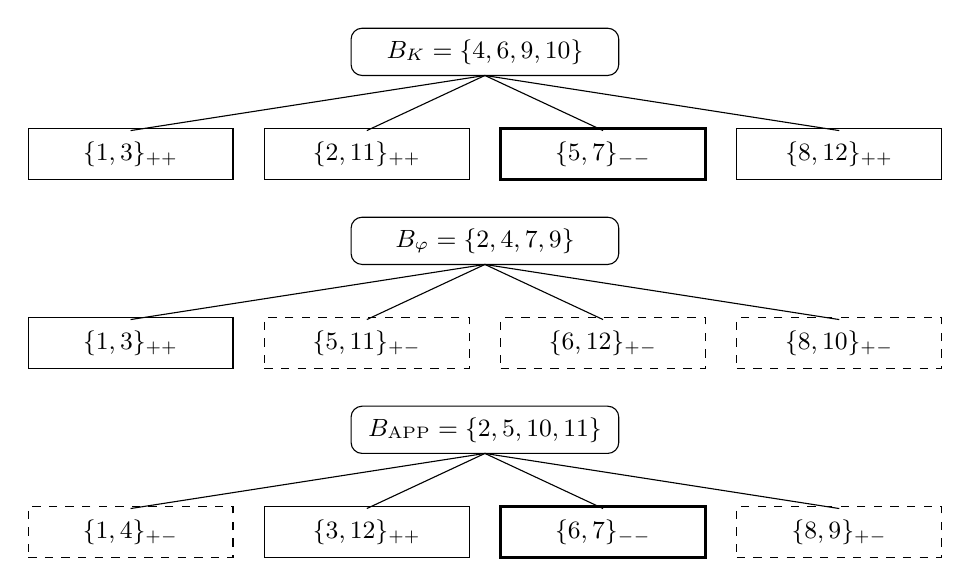
\begin{tikzpicture}[x=1cm,y=1cm,every node/.style={font=\small},
 core/.style={draw,rounded corners,minimum width=3.4cm,minimum height=.6cm},
 petal/.style={draw,minimum width=2.6cm,minimum height=.65cm}]
\foreach \y/\name in {0/{B_K=\{4,6,9,10\}},
 -2.4/{B_\varphi=\{2,4,7,9\}},-4.8/{B_{\rm APP}=\{2,5,10,11\}}}
 {\node[core] at (0,\y) {\(\name\)};
  \foreach \x in {-4.5,-1.5,1.5,4.5}
    {\draw (0,\y-.3)--(\x,\y-1);}}
\node[petal] at (-4.5,-1.3) {\(\{1,3\}_{++}\)};
\node[petal] at (-1.5,-1.3) {\(\{2,11\}_{++}\)};
\node[petal,very thick] at (1.5,-1.3) {\(\{5,7\}_{--}\)};
\node[petal] at (4.5,-1.3) {\(\{8,12\}_{++}\)};
\node[petal] at (-4.5,-3.7) {\(\{1,3\}_{++}\)};
\node[petal,dashed] at (-1.5,-3.7) {\(\{5,11\}_{+-}\)};
\node[petal,dashed] at (1.5,-3.7) {\(\{6,12\}_{+-}\)};
\node[petal,dashed] at (4.5,-3.7) {\(\{8,10\}_{+-}\)};
\node[petal,dashed] at (-4.5,-6.1) {\(\{1,4\}_{+-}\)};
\node[petal] at (-1.5,-6.1) {\(\{3,12\}_{++}\)};
\node[petal,very thick] at (1.5,-6.1) {\(\{6,7\}_{--}\)};
\node[petal,dashed] at (4.5,-6.1) {\(\{8,9\}_{+-}\)};
\end{tikzpicture}
\caption{Comparaison des trois étoiles. Chaque connexion représente
l'union du quadruplet supérieur avec une paire ; les douze hexades
complètes figurent dans le tableau~\ref{star27:tabla-tres}. Le contour
épais signale les paires négatives et le contour discontinu les paires mixtes.
Les connexions représentent l'incidence.}
\label{star27:figura}
\end{figure}

\begin{proposition}[Couplage de la couronne, de l'incidence et du signe]
\label{star27:acoplamiento}
Pour le registre dodécaphasique préalablement construit,
\[
B_K=\{i:K_i\geq729\}=H_e\cap P_\pi=\{4,6,9,10\}.
\]
L'unique hexade \(H\in\mathcal H\) qui satisfait
\(H\cap P_\pi=B_K\) est \(H_e\). De plus,
\[
H^-_\alpha=B_K\sqcup\{5,7\},\qquad
(B_\varphi\setminus B_K)\cap H^-_\alpha=\{7\}.
\]
\end{proposition}

\begin{proof}
Le registre
\(K=(234,543,140,729,659,824,621,58,914,794,146,601)\)
dépasse ou atteint \(729\) précisément aux quatre positions
indiquées. Sa comparaison avec les supports prouve la première
égalité. Une hexade dont l'intersection est \(B_K\) doit appartenir à
l'étoile de \(B_K\) ; parmi ses quatre paires, seule \(\{1,3\}\) est
disjointe de \(P_\pi\). Cela prouve l'unicité relative de \(H_e\).
Le tableau identifie la paire négative \(\{5,7\}\). Enfin,
\(B_\varphi\setminus B_K=\{2,7\}\), et les signes
\(s_2=297>0\), \(s_7=-3<0\) déterminent le pivot \(7\).
\end{proof}

Le quadruplet, le signe et la normalisation conservent des fonctions distinctes. L'incidence fixe la complétion \(H^-_\alpha\) ; le relèvement archimédien de la cochaîne complète utilise en outre les grandeurs, l'ordre positionnel et les retenues déjà démontrés dans la clôture de \(\alpha\). Cette composition explique comment une même généalogie produit une lecture géométrique de frontière et une lecture numérique.

\subsection{Classification polarisée des 495 quadruplets}
\label{star27:clasificacion}

\begin{theorem}[Recensement des signatures et restriction régionale]
\label{star27:censo}
Les \(495=\binom{12}{4}\) quadruplets se répartissent selon le tableau
\ref{star27:tabla-censo}. La dernière colonne compte les hexades
\(H\) avec \(|H\cap P_\pi|=4\), classées selon
\(\nu(H\cap P_\pi)\).
\end{theorem}

\begin{table}[htbp]
\centering
\begin{tabular}{ccc}
\toprule
\(\nu=(n_{++},n_{--},n_{+-})\)&Quadruplets&Hexadas regionales\\
\midrule
\((3,1,0)\)&15&9\\
\((1,3,0)\)&15&0\\
\((2,2,0)\)&45&9\\
\((1,1,2)\)&180&18\\
\((1,0,3)\)&120&18\\
\((0,1,3)\)&120&0\\
\midrule
Total&495&54\\
\bottomrule
\end{tabular}
\caption{Classification complète et restriction au support \(P_\pi\).
Les deux colonnes comptent des objets distincts : quadruplets et hexades.}
\label{star27:tabla-censo}
\end{table}

\begin{proof}
La procédure suivante constitue une énumération exacte du domaine fini. On forme les \(3^6\) mots \(w\), on calcule \((w,wA_W)\) modulo \(3\) et on conserve leurs supports de poids six sans répétition ; on obtient ainsi \(\mathcal H\), avec \(132\) éléments. Pour chaque \(B\in\binom{[12]}4\), on forme \(\mu_W(B)\), on compte les intersections de ses quatre paires avec \(H^-_\alpha\) et on incrémente l'entrée de la signature résultante. Les six compteurs sont \(15,15,45,180,120,120\). Leur somme est \(495\), et chaque quadruplet n'est traité qu'une seule fois. Pour la dernière colonne, on parcourt les \(132\) hexades, on retient les \(54\) dont l'intersection est de taille quatre et on applique à cette intersection la même fonction \(\nu\). Les opérations sont des comparaisons d'ensembles et de l'arithmétique dans \(\mathbb F_3\) ; le certificat reproductible conserve le tableau complet des entrées et des sorties.
\end{proof}

La signature \((3,1,0)\) appartient à quinze quadruplets. La
caractérisation du cadre régional utilise conjointement la couronne
de \(K\), l'intersection \(H_e\cap P_\pi\) et le signe de la
cochaîne, comme l'établit la proposition~\ref{star27:acoplamiento}.

\subsection{Rigidité du cadre ordonné de quatre supports}
\label{star27:rigidez}

Soit \(G_W=\langle\sigma_B:|B|=4\rangle\), déjà calculé dans la
proposition~\ref{exc:m12}. Pour une collection ordonnée de supports,
nous définissons
\[
\operatorname{Stab}_{G_W}(S_1,\ldots,S_r)
=\{g\in G_W:g(S_j)=S_j\ \text{pour tout }j\}.
\]
Chaque support est conservé individuellement ; les permutations internes
de ses points restent permises.

\begin{theorem}[Rigidité conjointe des quatre incidences]
\label{star27:marco}
Les stabilisateurs ont les ordres suivants :
\[
\begin{array}{l|r}
\text{données préservées}&\text{ordre}\\ \hline
H^-_\alpha&720\\
H^-_\alpha,\ 6&120\\
B_K&192\\
B_K,H^-_\alpha&48\\
B_K,H^-_\alpha,H_e&16\\
H^-_\alpha,H_e,H_\varphi&2\\
H^-_\alpha,H_e,H_\varphi,H_{\rm APP}&1
\end{array}
\]
Dans la deuxième ligne, le point \(6\) est également conservé.
En particulier,
\[
\operatorname{Stab}_{G_W}
(H^-_\alpha,H_e,H_\varphi,H_{\rm APP})=\{\operatorname{id}\}.
\]
\end{theorem}

\begin{proof}
On utilise la clôture par composition des six permutations
explicites de la proposition~\ref{exc:m12}. Sur ses \(95040\)
éléments, on évalue les prédicats \(g(S_j)=S_j\), conjointement avec
\(g(6)=6\) lorsque cela s'applique. Les sommes des indicatrices de
ces prédicats donnent, respectivement,
\(720,120,192,48,16,2,1\). L'identité satisfait toutes les
conditions ; le dernier cardinal prouve qu'elle est l'unique élément.
L'algorithme de clôture s'arrête par stabilité de l'ensemble,
et les filtres de stabilisation s'appliquent ensuite au groupe complet.
\end{proof}

Le tableau compare sept configurations marquées. Deux chaînes
d'inclusions utiles sont celles déterminées par
\((B_K)\), \((B_K,H^-_\alpha)\), \((B_K,H^-_\alpha,H_e)\),
et par
\((H^-_\alpha)\), \((H^-_\alpha,H_e,H_\varphi)\),
\((H^-_\alpha,H_e,H_\varphi,H_{\rm APP})\).
La rigidité finale exprime que le cadre régional ordonné fixe
complètement la liberté résiduelle au sein de \(G_W\). Son domaine est
l'action sur les douze positions ; le transport ultérieur vers les
réseaux et les algèbres conserve les applications propres à ces réalisations.

\subsection{Topologie finie de l'incidence et conservation de son domaine}
\label{star27:topologia}

Le complexe simplicial engendré par les \(132\) hexades a pour vecteur
de faces
\[
(f_0,f_1,f_2,f_3,f_4,f_5)=(12,66,220,495,792,132)
\]
et la caractéristique d'Euler \(\chi=12-66+220-495+792-132=331\). En effet, chaque ensemble de cinq points possède une extension hexadique unique ; tout sous-ensemble de cardinal inférieur appartient à l'un de ces ensembles, et les faces maximales sont les hexades.

Le graphe biparti entre quadruplets et hexades possède
\[
|V|=495+132=627,\qquad |E|=495\cdot4=132\cdot15=1980.
\]
Il est connexe. Soient \(H\) et \(H_*\) deux hexades distinctes ; leur
intersection comporte au plus quatre points, car l'extension
d'un quintuplet est unique. Choisissons un quadruplet \(B\subset H\)
qui contienne \(H\cap H_*\), et un point \(p\in H_*\setminus H\).
L'unique extension \(H'\) de \(B\cup\{p\}\) est reliée à
\(H\) par le chemin biparti \(H-B-H'\) et satisfait
\(|H'\cap H_*|>|H\cap H_*|\). En répétant l'opération, on
atteint \(H_*\) ; contenir cinq de ses points impose déjà
l'égalité. Tout quadruplet possède quatre hexades incidentes, de
sorte qu'il appartient également à cette composante unique.
Son premier nombre de Betti est donc
\[
\beta_1=|E|-|V|+1=1354.
\]
Le parcours exhaustif de l'incidence vérifie aussi la
connexité. Pour les paires non ordonnées d'hexades distinctes, le recensement
des tailles d'intersection est
\[
\begin{array}{c|rrrr}
|H\cap H'|&0&2&3&4\\ \hline
\#\{H,H'\}&66&2970&2640&2970 .
\end{array}
\]
La somme \(8646=\binom{132}{2}\) couvre toutes les paires.

Ces invariants décrivent le complexe et son graphe d'incidence.
Le micrographe de raccordements \(U_6=A|B\) conserve séparément ses
\(96\) sommets, \(234\) arêtes, six composantes et
\(\beta_1=234-96+6=144\). De même, la composition des
\(\sigma_B\) agit sur des positions d'incidence, tandis que
\(\Gamma_9\) transporte l'état TPK à mémoire. Cette précision
permet de relier les lectures au moyen de leurs applications effectives et de
conserver, à chaque niveau, les données utilisées par l'opération.
